\documentclass[
	a4paper
]{scrartcl}

%%% PACKAGES %%%

% PDF/A Compliance
\usepackage[a-2b]{pdfx}

% add unicode support and use german as language
\usepackage[utf8]{inputenc}
\usepackage[ngerman]{babel}

% Use Helvetica as font
\usepackage[scaled]{helvet}
\renewcommand\familydefault{\sfdefault}

% Better tables
\usepackage{tabularx}

% Better enumerisation env
\usepackage{enumitem}

% Use graphics
\usepackage{graphicx}

% Have subfigures and captions
\usepackage{subcaption}

% Be able to include PDFs in the file
\usepackage{pdfpages}

% Have custom abstract heading
\usepackage{abstract}

% Need a list of equation
\usepackage{tocloft}
\usepackage{ragged2e}

% Better equation environment
\usepackage{amsmath}

% Symbols for most SI units
\usepackage{siunitx}

\usepackage{csquotes}

% Clickable Links to Websites and sections
\usepackage{hyperref}

% Change page rotation
\usepackage{pdflscape}

% Symbols like checkmark
\usepackage{amssymb}
\usepackage{pifont}

\usepackage[absolute]{textpos}

%make figures stay where they belong
\usepackage{float}

% Change line spacing
\renewcommand{\baselinestretch}{0.9}

%%% PATH DEFINITIONS %%%
\graphicspath{{./img/}}

%%% DOCUMENT %%%

\begin{document}

\pagenumbering{gobble}

\begin{textblock*}{5cm}[0,0](15cm,0.7cm)
	\includegraphics[keepaspectratio,width=5cm]{img/HSLU_Logo}
\end{textblock*}

\vspace*{2cm}

\noindent
\textbf{\LARGE{Erfassung von Anzahl und Position von Personen in Sitzungszimmer}} \\

\vspace{0.5em}

\bgroup
% Remove padding of the table
\setlength\tabcolsep{0cm}

% Table itself
\begin{large}
\noindent
\begin{tabularx}{\textwidth}{p{5cm}X}
	\textbf{Themenbereiche:} & Infrarot, Objekterkennung, CNN\\
	\textbf{Studierende:} & Pascal Stalder\\
	\textbf{Betreuungsperson:} & Olivier Steiger\\
	\textbf{Co-Betreuungsperson:} & Martin Camenzind\\
	\textbf{Experte:} & Stefan Chiappori\\
	\textbf{Auftraggebende:} & iHomeLab\\
	\textbf{Keywords:} & Infrarot, People counting, Objekterkennung, Smart Office\\
\end{tabularx}
\end{large}
\egroup

\section{Aufgabenstellung}
Gebäudesteuerungen sollen in Zukunft mehr auf die Belegungen und das Verhalten der Bewohner eingehen, anstatt einem fixen Schema zu folgen. Voraussetzung dafür ist, dass die Steuerung, die Belegung und das Verhalten der Bewohner kennt.\\
Dafür soll in dieser Diplomarbeit das Potential kostengünstiger thermischer Kamerasystemen, zur Erfassung des Nutzerverhaltens in Büroräumen evaluiert werden. Mittels State-of-the-Art Bildanalyse und Deep-Learning soll versucht werden, die Belegung und den Personenfluss eines Sitzungszimmers zu bestimmen.\\
Ein Sitzungsraum der Hochschule Luzern in Horw wurde dafür mit zwei Infrarotkameras ausgerüstet. Zusätzlich steht eine herkömmliche Kamera als Referenz zur Verfügung.\\
\\
Ziel dieser Arbeit ist es ein System zu entwickeln, welches die Anzahl und Position der Personen auf einem Infrarotbild bestimmt. Dabei soll aufgezeigt werden, welche Schwierigkeiten bei der Entwicklung eines solchen Systems beachtet werden müssen und wie diese überwunden werden können.
Insbesondere sind folgende Resultate vorzulegen:
\begin{itemize}[noitemsep]
	\item Zwei implementierte Algorithmen zur Lösung der Problemstellung.
	\item Eine ausführliche Evaluation des Systems.
	\item Möglichkeiten und Vorschläge zur Lösung der aufgetretenen Schwierigkeiten und zur Verbesserung des Systems.
\end{itemize}

\vspace{0.5em}
\noindent
\begin{textblock*}{5cm}[0,0](14.93cm,277mm)
	\includegraphics[keepaspectratio,width=5cm]{img/FHZ_Logo}
\end{textblock*}

\newpage

\begin{textblock*}{5cm}[0,0](15cm,0.7cm)
	\includegraphics[keepaspectratio,width=2.7cm]{img/HSLU_Logo_Header}
\end{textblock*}

\section{Ergebnisse}
Wie in der Aufgabenstellung beschrieben wurden zwei passende Algorithmen implementiert. Es wurde ein Convolutional Neural Network(CCN) trainiert und als Referenz dazu eine relativ simple Threshold-Methode. Diese beiden Algorithmen wurden getestet und evaluiert. Dabei zeigte sich, dass beide Algorithmen ein relativ gutes Ergebnis erzielen. Die grössten gefundenen Schwierigkeiten für das System sind wie erwartet fremde Wärmequellen aber auch Isolierende Kleider. Dabei stellen Laptops die in Intensivem Betrieb sind, von Personen erwärmte Stühle und Radiatoren die grössten Probleme. Die Threshold-Methode kann diese, wenn sie in einem ählichen Wärmebereich befinden wie Menschen, ab einer gewissen Grösse nicht von Personen unterscheiden. Das CNN hat ähnliche Probleme mit diesen Wärmequellen, es konnte jedoch gezeigt werden, dass mit spezifischem Training das CNN so erweitert werden kann, dass es diese nicht mehr als Personen erkennt. 

\begin{figure}[H]
	\begin{subfigure}{\linewidth}
		\centering
		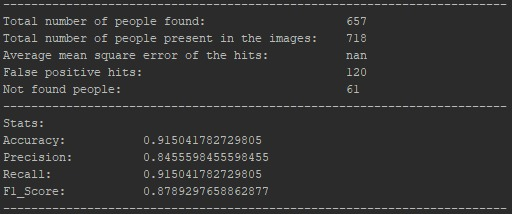
\includegraphics[keepaspectratio, height=4cm]{cnnSummary}
		\caption{Zusammenfassung der CNN Ergebnisse}
		\label{fig:cnnSummary}		
	\end{subfigure}
	\begin{subfigure}{\linewidth}
		\centering
		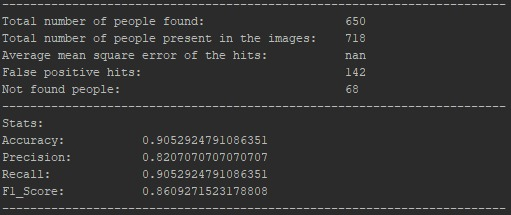
\includegraphics[keepaspectratio, height=4cm]{threshSummary}
		\caption{Zusammenfassung der Ergebnisse der Threshold-Methode}
		\label{fig:threshSummary}		
	\end{subfigure}
\end{figure}

\section{Lösungskonzept}
Das ganze Projekt wurde iterativ-inkrementell durchgeführt. Da es sich um ein Exploratives Projekt handelte, wurden Ideen in kleinem Rahmen umgesetzt, evaluiert und wenn sie sich bewährten weiterentwickelt. Das Projekt teilte sich darüber hinaus in drei Phasen auf. Die Intialrecherche, die Implementierung der ausgewählten Algorithmen und die Evaluation des Systems.\\
da die Auflösung der Bilder mit 80x64 Pixel sehr klein ist 

\begin{textblock*}{5cm}[0,0](14.93cm,277mm)
	\includegraphics[keepaspectratio,width=5cm]{img/FHZ_Logo}
\end{textblock*}

\newpage

\begin{textblock*}{5cm}[0,0](15cm,0.7cm)
	\includegraphics[keepaspectratio,width=2.7cm]{img/HSLU_Logo_Header}
\end{textblock*}


\section{Spezielle Herausforderungen}
Eine Herausforderung in dieser Aufgabe war es die Bilder von Infrarotkameras zu erhalten. Denn sie boten nicht, wie sonst üblich, eine Webschnittstelle an, sondern konnten nur über UDP-Broadcasts angesprochen werden. Zudem konnte man zwar Einzelbilder anfordern, diese waren qualitativ aber sehr schlecht, weshalb die Schnittstelle nachträglich auf die Verwendung von Streams abgeändert werden musste.
Zudem war das finden einer guten Komposition des CNN's schwierig. Dies, weil die meisten Papers zwar aussagen, dass sie ein CNN verwenden, aber nicht wie dieses aufgebaut ist. Auch wurden insgesammt nicht viele Quellen gefunden die sich in dieser Art mit Bilder von so niedriger Auflösung befassen.

\section{Ausblick}
Um ein solche System fertig aufzubauen müsste hauptsächlich noch in verbessertes Training, des CNN's inverstiert werden. Dies zeigt eine Vielversprechende Basis und sollte mit den richtigen Trainigsdaten und einer passenden Konfiguration in der Lage sein zuverlässig, Personen und deren Position zu erkennen.\\
Soll das System breiter angewendet werden und in verschiedenen Umfelder zum Einsatz kommen, muss genau analysiert werden, ob die Auflösung der Kameras ausreicht. Denn wie auf dem Bild zu sehen steht sehr wenig Information zur Verfügung. Sobald Personen grosse Unterschiede in Temperatur und Haltung aufweisen, wird es schwierig diese eindeutig zu Identifizieren.

\begin{figure}[H]
	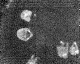
\includegraphics[height=5cm]{exampleIRImage}
\end{figure}

\vspace{0.5em}
\noindent
\begin{textblock*}{5cm}[0,0](14.93cm,277mm)
	\includegraphics[keepaspectratio,width=5cm]{img/FHZ_Logo}
\end{textblock*}
\end{document}
